\section{Resolución del corto}
\begin{enumerate}
    \item La productividad marignal 
    \item Qué necesita el empresario: nada mas que una buena idea
    \item El numero de damba, la gente ya no aprecia las cosas que les dan porque por eso la ayuda social tiende a fracasar ya que a las personas les da igual
    \item Hay muchas, la que puse fue el carácter creativo de la función empresarial.
\end{enumerate}

\section{Noticia}
``Dos pinos enfrenta denuncia de competencia desleal en El Salvador'', se diferencia en costa rica y en el salvador, es mas caro en costa rica. No se consideró dumping, la competencia es justa. Se quería imponer un arancel.

\section{Discusión de clase}
En el caso de la leche si se imponen barreras como aranceles o en nombre de la salud se imponen barreras implícitas, muchas veces las barreras arancelarias son producto de cabildeo, caso de incaparina y la leche; cada país tiene sus mañas de aranceles, es un catástrofe económico.

\section{Derecho, dinero y cáculo económico}
\begin{itemize}
    \item Muchos empresarios se refieren al estado como el socio invisible. 
    \item Se necesita legislación para la empresarialidad.
    \item Arbitrage judicial: es una corte privada.
    \item Hay pocos incentivos de empresarialidad si las acciones de los individuos no se someten a un comportamiento específico.
    \item David Hume; 
    
    \item El derecho de propiedad:
    \begin{itemize}
        \item Derecho exclusivo de posesión.
        \item transmisión mediante a patente.
        \item Cumplimiento de las promesas(contratos).
    \end{itemize}
    
    \item \textbf{\emph{Ejemplo:}} cuando una persona invade el terreno de otra muchos lo que hacen es decir que están cortando arboles 
    \item \textbf{\emph{Ejemplo:}} Los 8,000 pepinos y el carro.
    \item Cualquier cosa que esté en contrato es principio de ley. Si no existe la legislación no aparecen los empresarios.
    \item Si los agentes no se someten a la legislación la empresarialidad no aparece.
\end{itemize}

\section{Arbitraje y especulación}
\begin{itemize}
    \item La empresarialidad puede ser ejercida en el presente y futuro. \textbf{Comprar barato para vender caro}. 
    \item Arbitraje es ejercer la empresarialidad en un lapso temporal.
    \item \textbf{\emph{Ejemplo:}} Si se imponen sanciones en Iran qué pasa con el petrolio \emph{\textbf{Respuesta}:se dispara el precio.}
    \item La mayor parte de empresarios tienden a ser especuladores, intentan anticipar una subida de precio, o una bajada de precio para afinar su estrategia.
    \item \textbf{\emph{Ejemplo:}} cuando uno pide una hipoteca uno está positivo en vivienda pero corto en dinero, se pide una hipoteca (tambien el que adquirió la hipoteca quere que su casa se devalúe).
    \item La especulación es que intentas anticipar precios futuros para afinar la estrategia.
\end{itemize}

\begin{figure}[htbp]
    \centering
    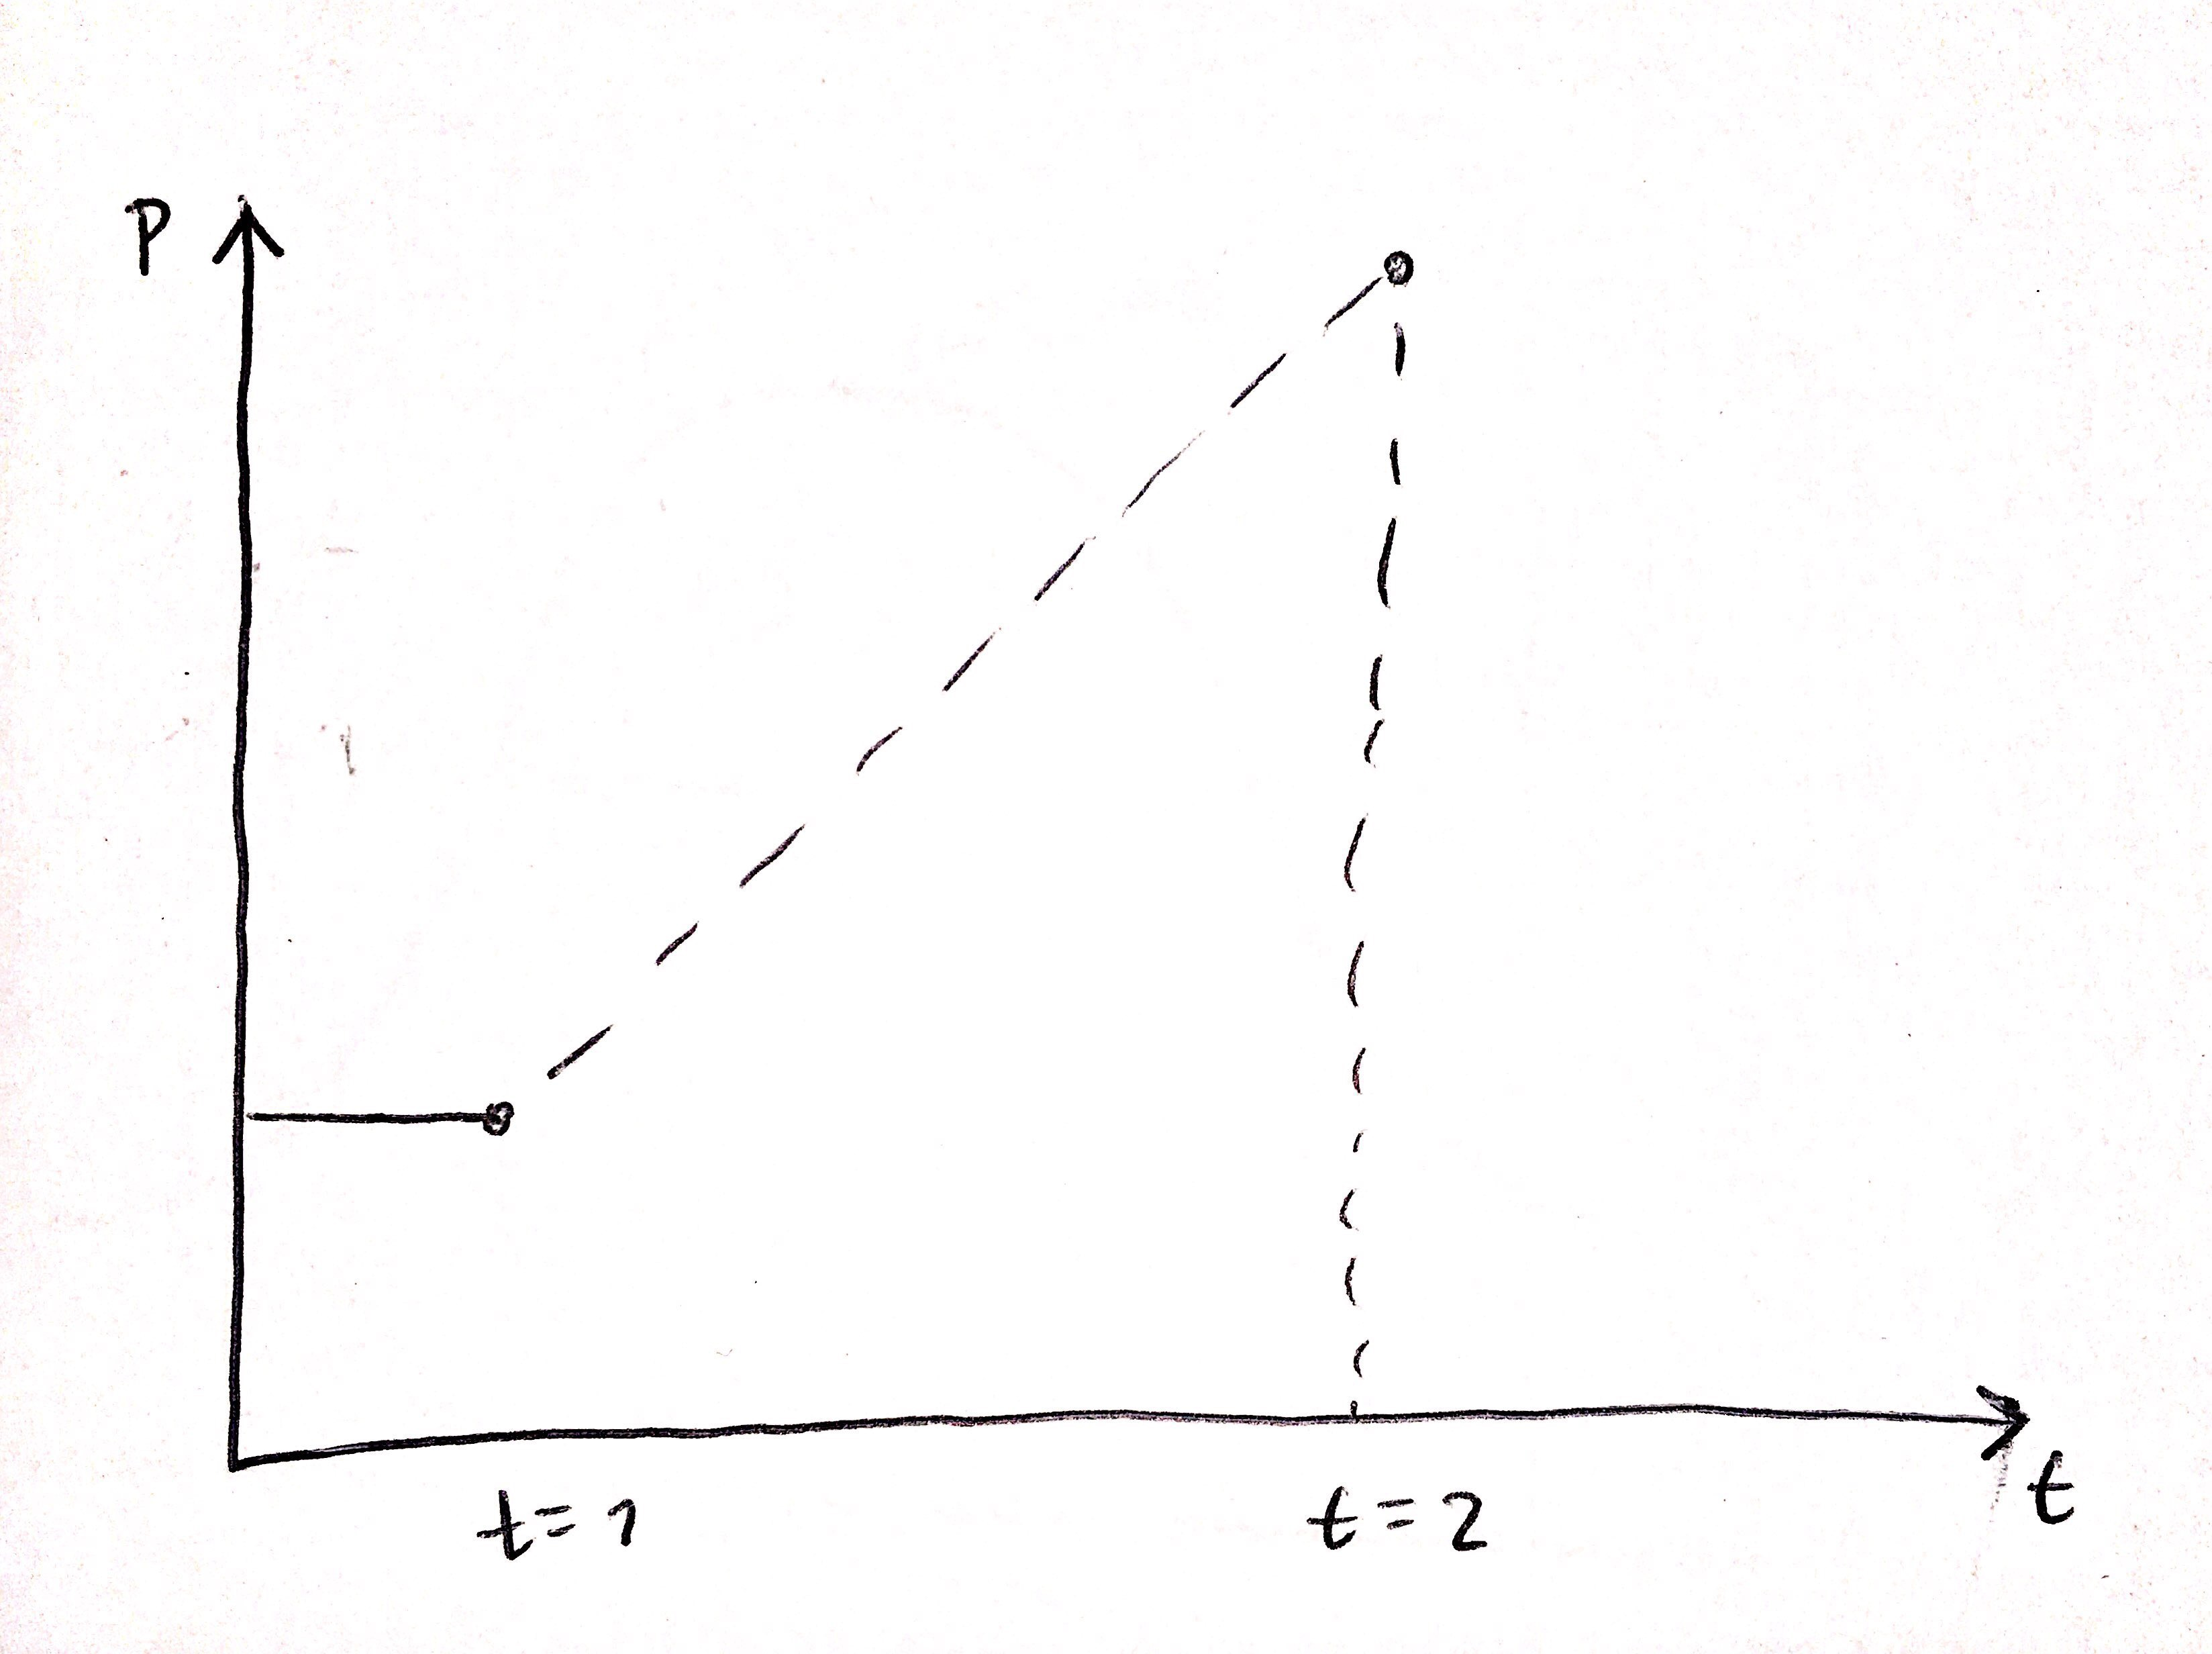
\includegraphics[width=8cm]{Classes/Images/2019-08-05-01.jpg}
    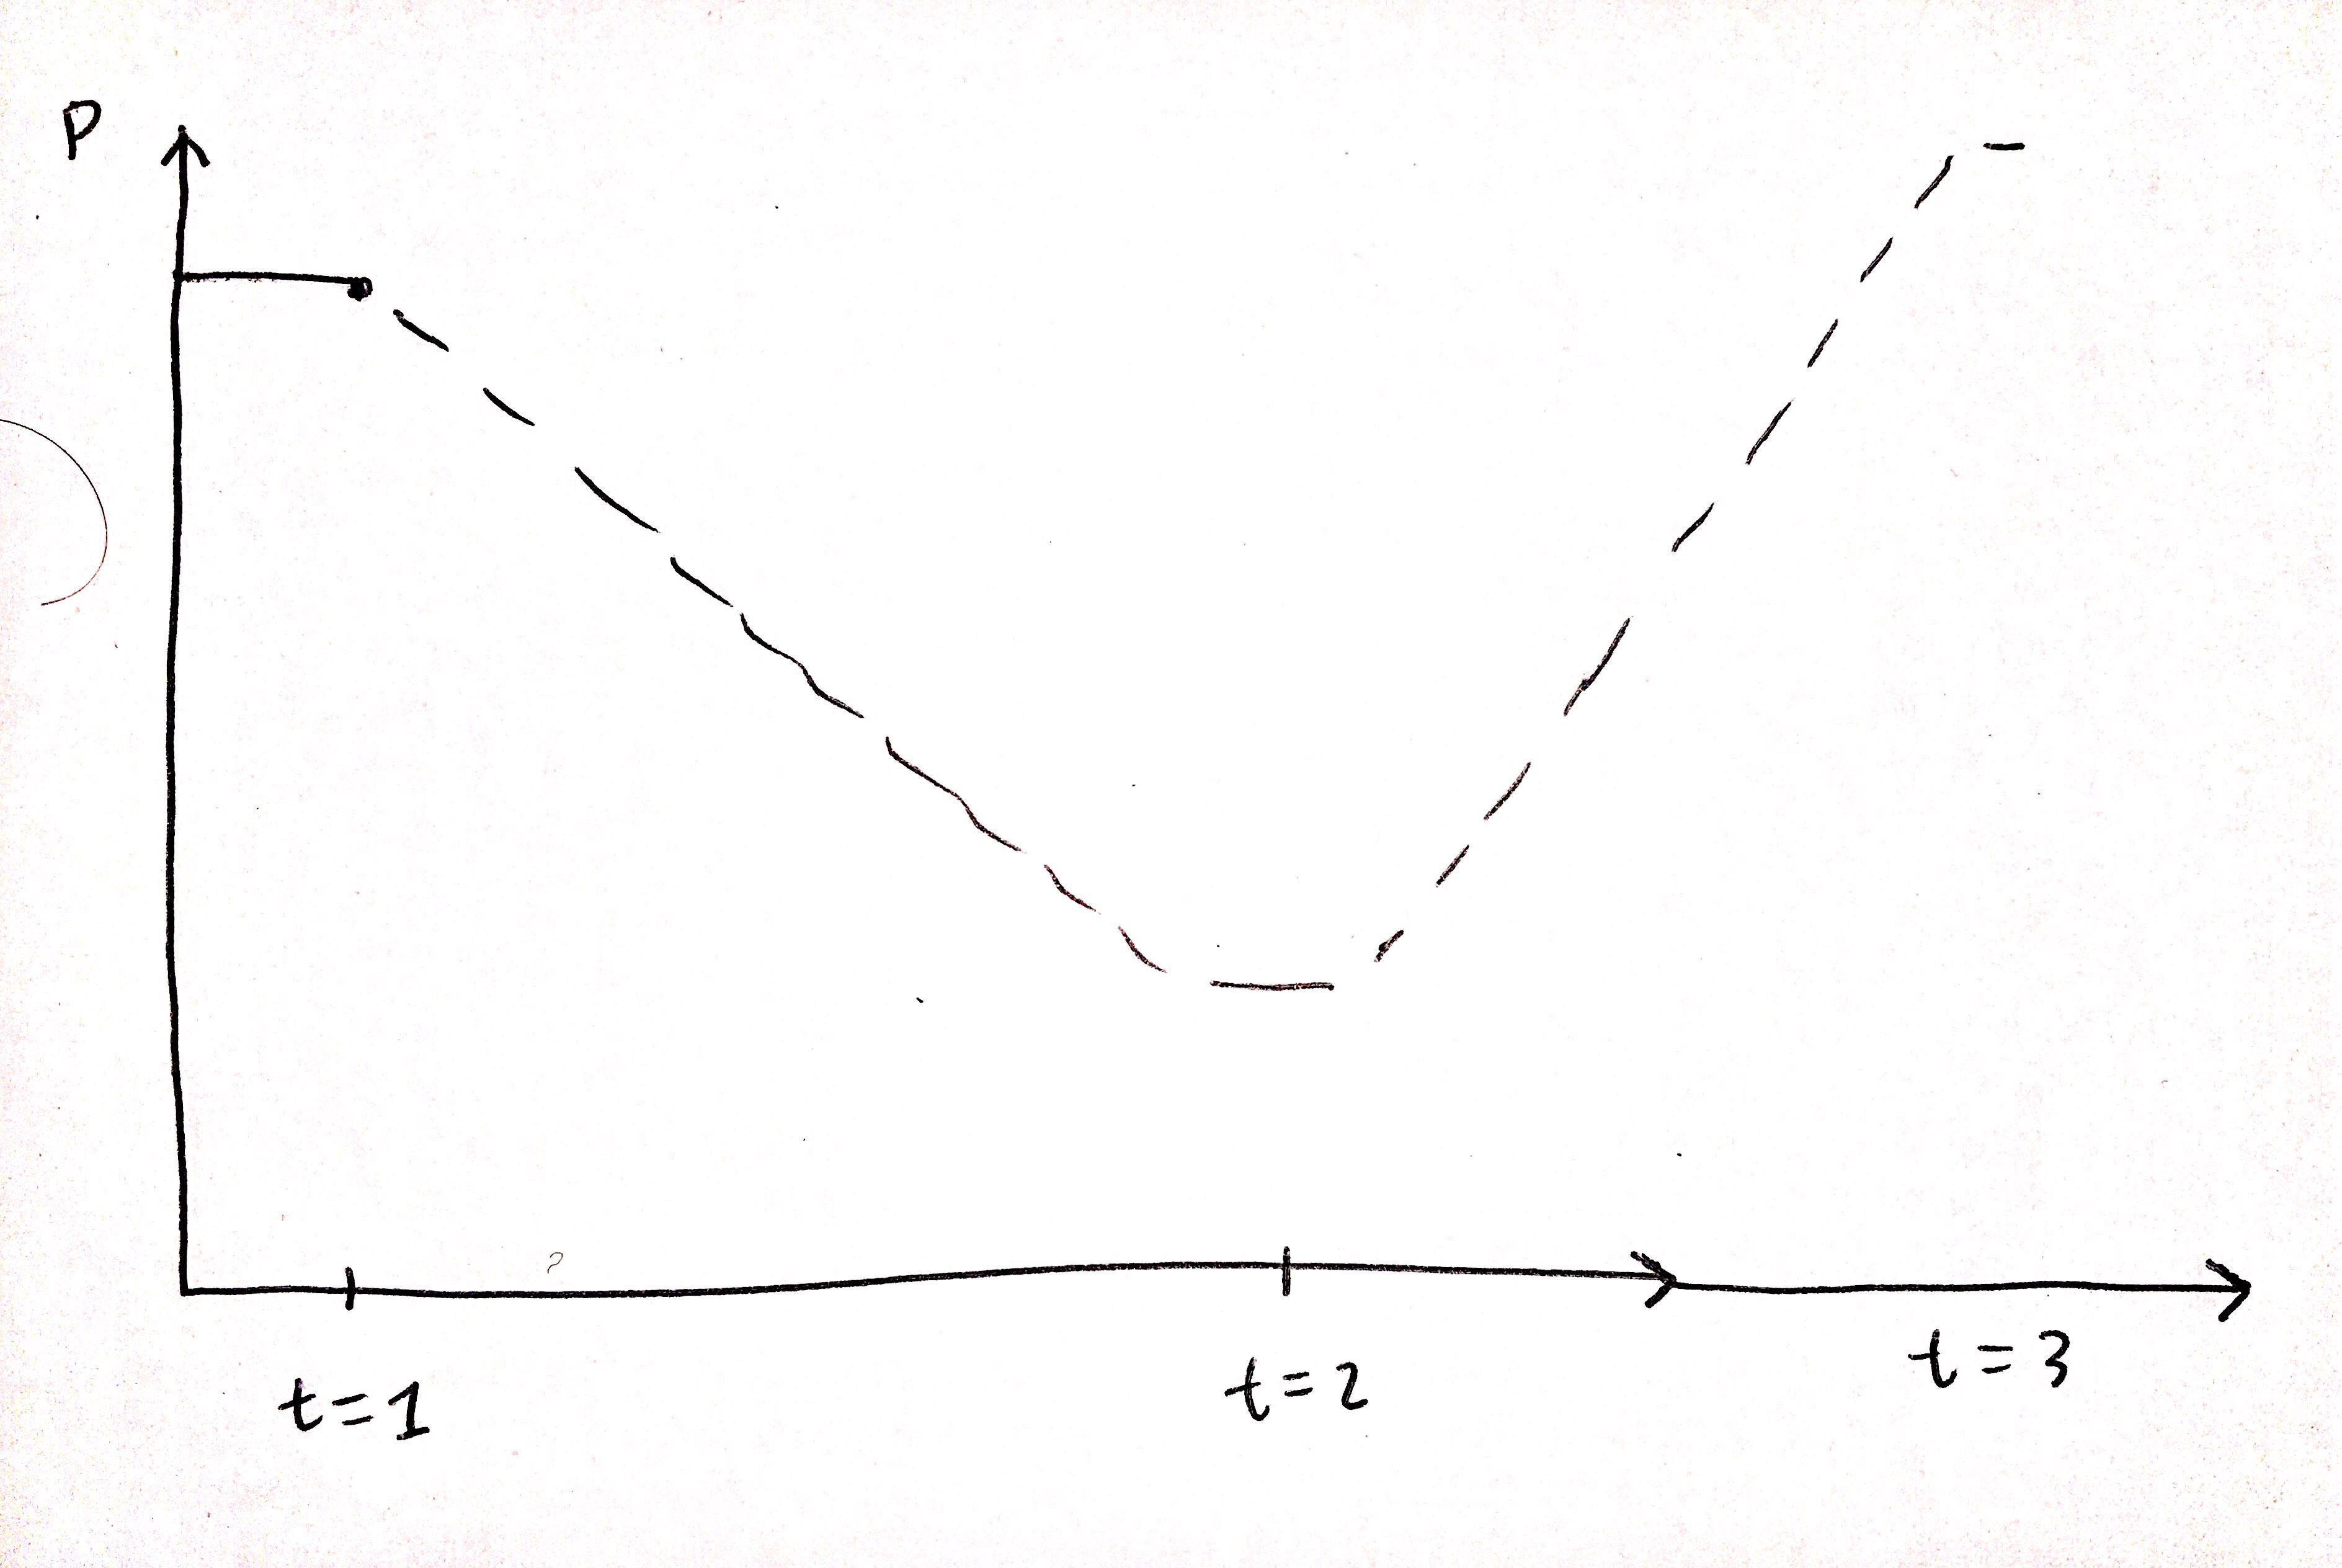
\includegraphics[width=8cm]{Classes/Images/2019-08-05-02.jpg}
    \caption{Especulación a través del tiempo}

    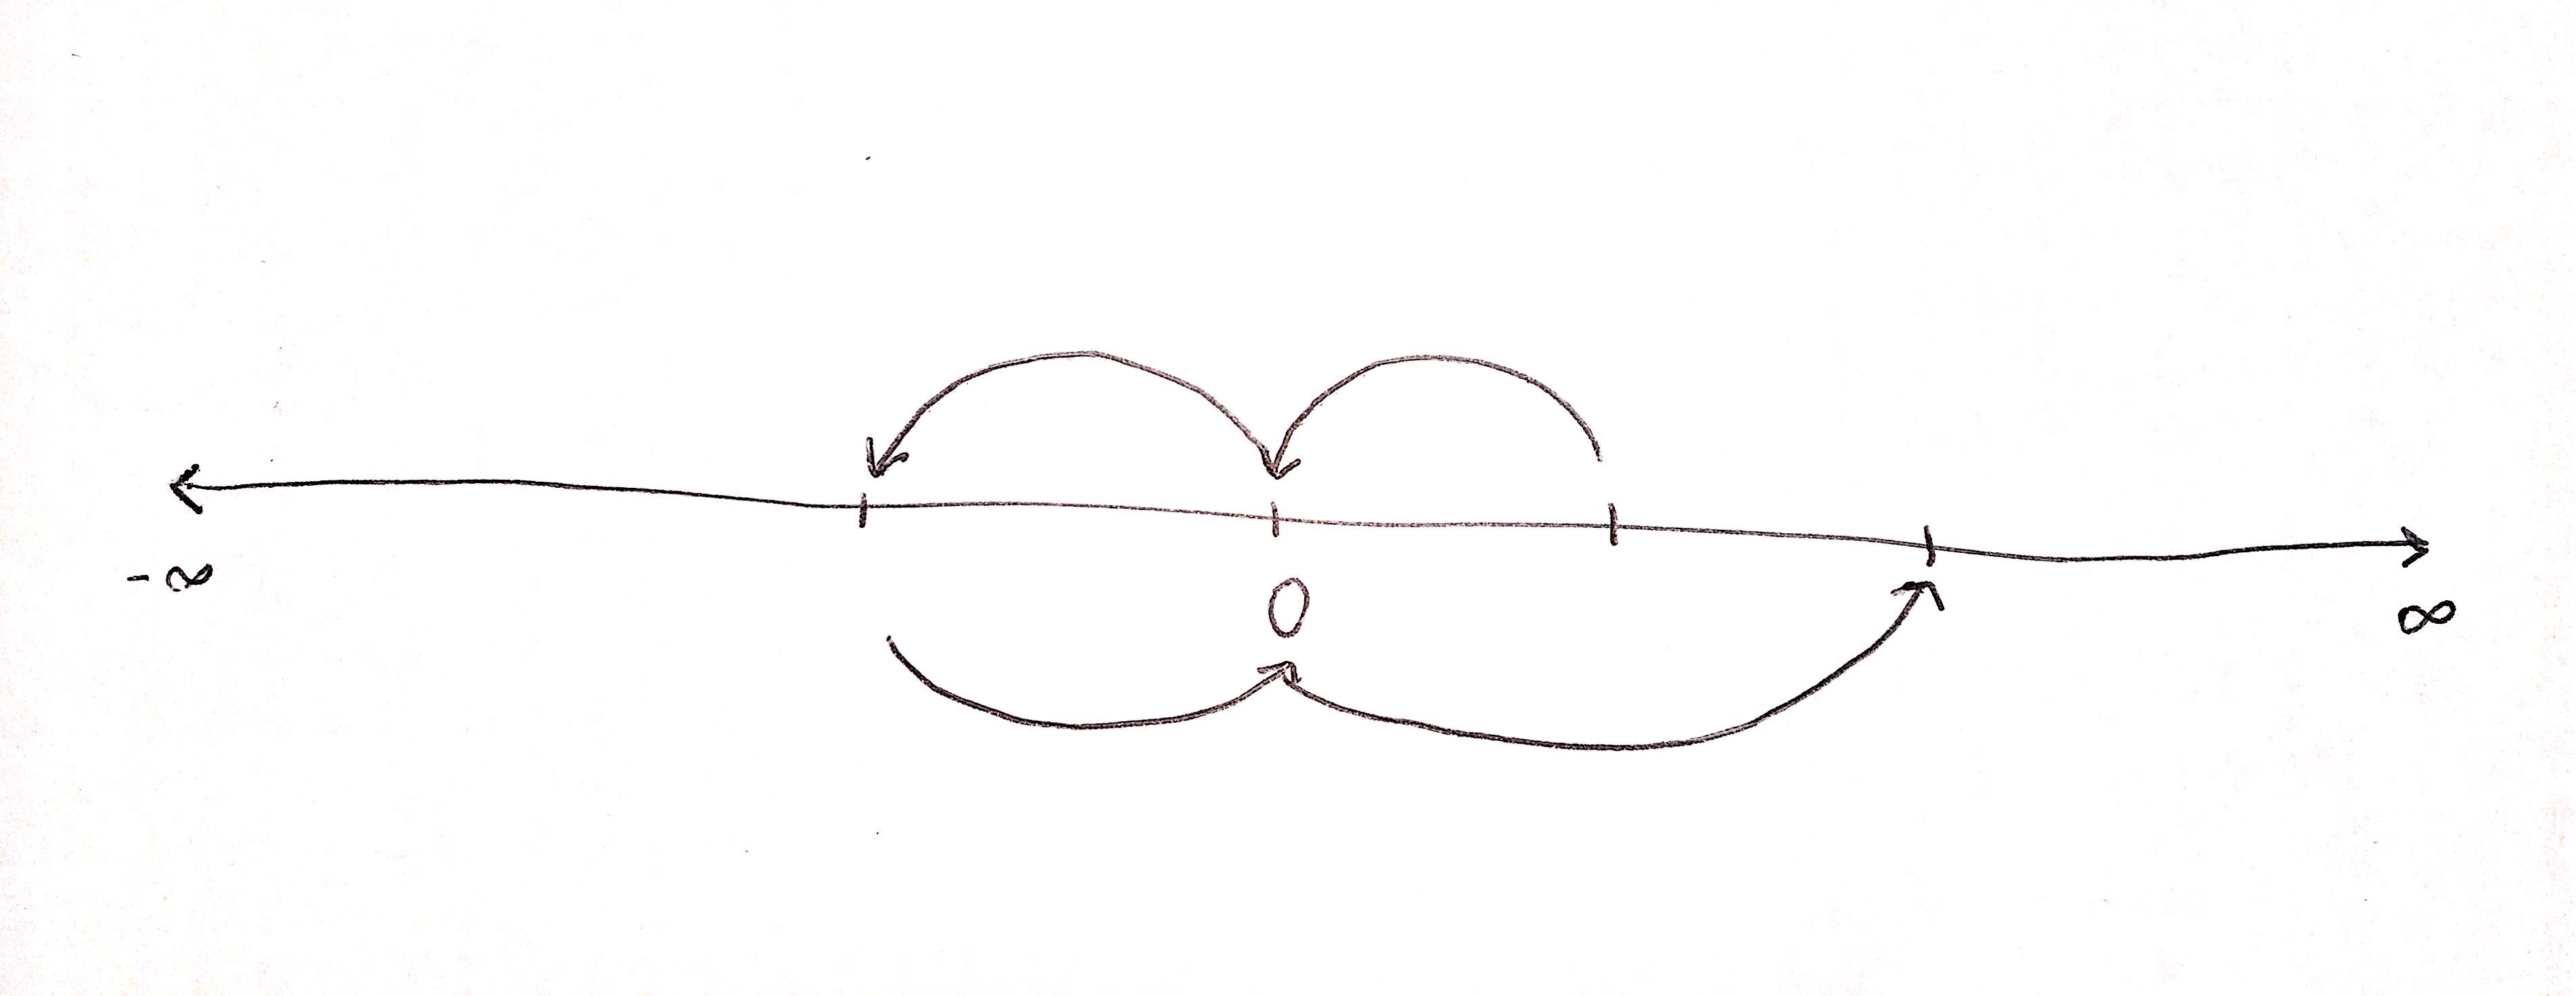
\includegraphics[width=12cm]{Classes/Images/2019-08-05-03.jpg}
    \caption{Me pongo corto para vender lo que no tengo y genero valor mientras especulo}
    \label{}
\end{figure} 


\section{Competencia y función empresarial}
\begin{itemize}
    \item La competencia es una rivalidad, una concurrencia hacia un bien o servicio.
    \item Básicamente es la competencia es un proceso de rivalidad por obtener oportunidades de ganancia. \emph{\textbf{Paréntesis:}Las oportunidades de ganancia viene de coordinar recursos que tienen unas personas y quieren otras.} \textbf{\emph{Ejemplo:}} el petroleo de Tejas. 
    \item El proceso de competencia tiende a destruir los beneficios por la \textbf{imitación}.
    \item \textbf{\emph{Ejemplo:}} dos pinos y su competencia.
    \item \textbf{Nos preguntamos:} ¿Se pueden agotar las oportunidades de ganancias? ¿Puede ocurrir? \emph{\textbf{Respuesta}:no, las necesidades son subjetivas, la innovación no permite que se agoten a cero las oportunidades de ganancia, esto y otros factores}, \textbf{\emph{Ejemplo:}} el puerto el fin de semana, hace un siglo ir al puerto era asunto de 4 días de viaje. 
\end{itemize}

\section{Division de conocimiento y orden extensivo de cooperación social}
\begin{itemize}
    \item La capacidad intelectual del ser humano ha permanecido constante
    \item Hayek: cuando se aprende algo se deja de aprender otra cosa.
    \item Lo importante no es dividir el trabajo, es dividir el conocimiento. \textbf{el recurso primordial en economia son ideas}.
\end{itemize}


\section{Socialismo}
\begin{itemize}
    \item \emph{Citación:``Toda agresión institucional que agrede la empresarialidad."}
    \item Intentos de restringir: usualmente se hacen en nombre de ``mejorar el procedimiento social''. Son muy bien intencionadas pero por ser bestia se producen más problemas.
\end{itemize}
